\apendice{Manual de especificación del diseño}
En este trabajo se ha realizado la implementación de diferentes modelos epidemiológicos deterministas utilizando diversas herramientas del entorno de MATLAB.
\section{Planos}
Aunque no se han elaborado planos arquitectónicos formales, se han utilizado diagramas de bloques en \textbf{Simulink} para representar los distintos modelos epidemiológicos (SI, SIS, SIR, SEIR, SIRV y SEIR). 
Estos diagramas no constituyen planos técnicos tradicionales, pero permiten visualizar de forma clara y esquemática la estructura dinámica de cada modelo, mostrando las interacciones entre los compartimentos y facilitando la comprensión y simulación del sistema.

A continuación se muestran los diagramas de bloques para cada modelo.

\textbf{Modelo SI} representado en la figura \ref{fig: diagrama de bloques en Simulink para el modelo SI}, representa la dinámica básica entre individuos susceptibles e infectados, asumiendo que una vez infectados, permanecen en ese estado sin recuperación.
\begin{figure}[H]
        \centering
        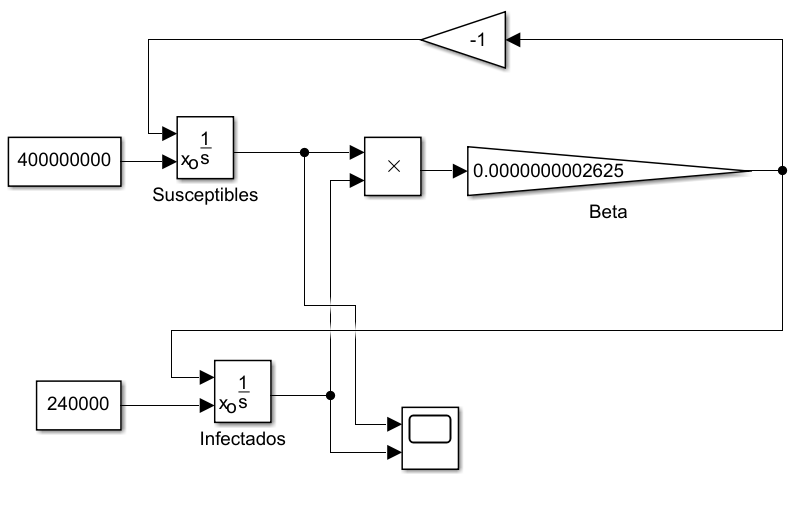
\includegraphics[width=0.7\textwidth]{img/modelo_SI.png}
        \caption{Diagrama de bloques en Simulink para el modelo SI}
        \label{fig: diagrama de bloques en Simulink para el modelo SI}
        \vspace{0.5cm} % Ajusta el espacio vertical entre la imagen y el texto
\end{figure}

\textbf{Modelo SIS} representado en la figura \ref{fig: diagrama de bloques en Simulink para el modelo SIS}, contempla que los individuos infectados pueden recuperarse pero sin adquirir inmunidad, volviendo al estado susceptible.
\begin{figure}[H]
        \centering
        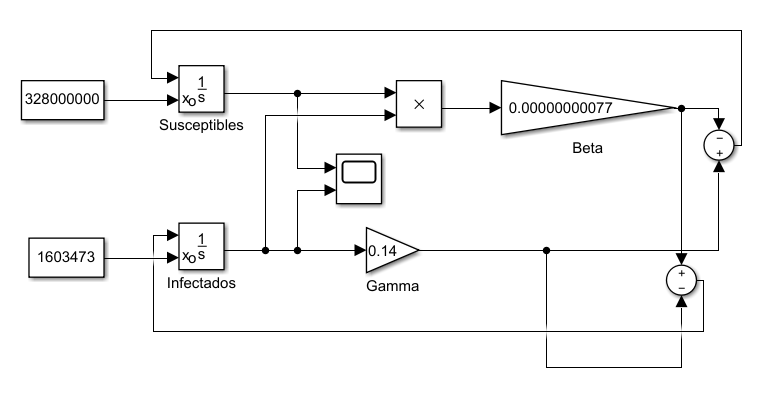
\includegraphics[width=0.7\textwidth]{img/modelo_SIS.png}
        \caption{Diagrama de bloques en Simulink para el modelo SIS}
        \label{fig: diagrama de bloques en Simulink para el modelo SIS}
        \vspace{0.5cm} % Ajusta el espacio vertical entre la imagen y el texto
\end{figure}

\textbf{Modelo SIR} representado en la figura \ref{fig: diagrama de bloques en Simulink para el modelo SIR}, los individuos susceptibles pueden infectarse, pasar a infectados y posteriormente recuperarse con inmunidad permanente.


\begin{figure}[H]
        \centering
        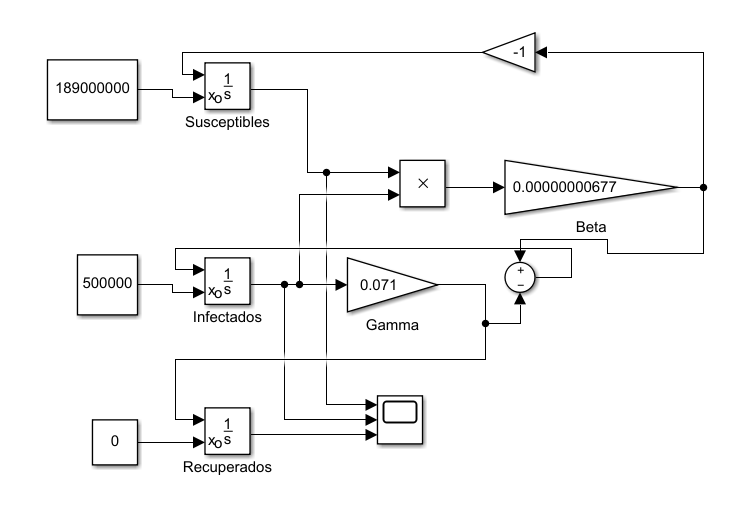
\includegraphics[width=0.7\textwidth]{img/modelo_SIR.png}
        \caption{Diagrama de bloques en Simulink para el modelo SIR}
        \label{fig: diagrama de bloques en Simulink para el modelo SIR}
        \vspace{0.5cm} % Ajusta el espacio vertical entre la imagen y el texto
\end{figure}



\textbf{Modelo SEIR} representado en la figura \ref{fig: diagrama de bloques en Simulink para el modelo SEIR}, extensión del modelo SIR que incluye una fase de exposición, donde los individuos están infectados pero no son contagiosos durante un período de incubación.
\begin{figure}[H]
        \centering
        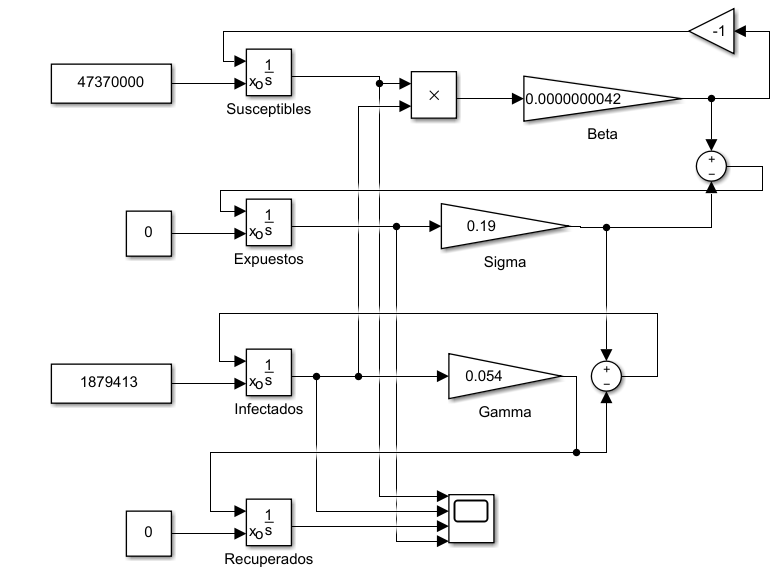
\includegraphics[width=0.7\textwidth]{img/modelo_SEIR.png}
        \caption{Diagrama de bloques en Simulink para el modelo SEIR}
        \label{fig: diagrama de bloques en Simulink para el modelo SEIR}
        \vspace{0.5cm} % Ajusta el espacio vertical entre la imagen y el texto
\end{figure}

\textbf{Modelo SIRV} representado en la figura \ref{fig: diagrama de bloques en Simulink para el modelo SIRV}, modelo SIR que incorpora la vacunación como una vía adicional para pasar de susceptibles a inmunes sin pasar por la infección.
\begin{figure}[H]
        \centering
        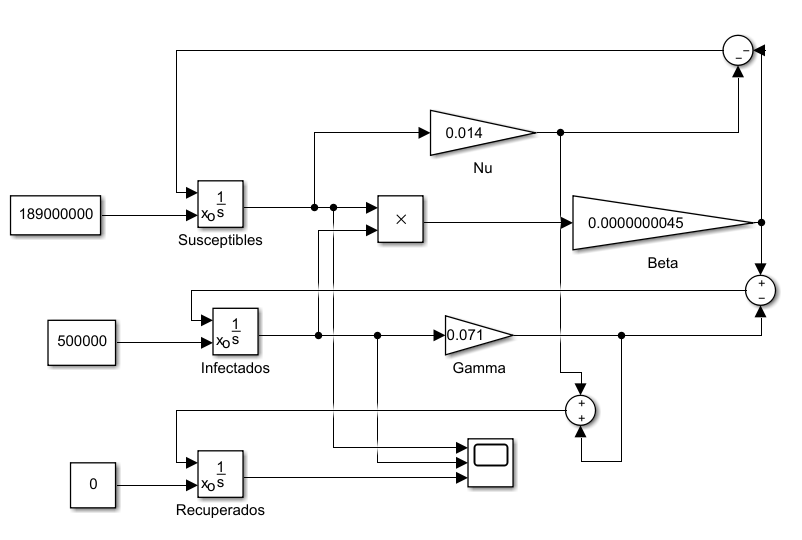
\includegraphics[width=0.7\textwidth]{img/modelo_SIRV_inicio.png}
        \caption{Diagrama de bloques en Simulink para el modelo SIRV}
        \label{fig: diagrama de bloques en Simulink para el modelo SIRV}
        \vspace{0.5cm} % Ajusta el espacio vertical entre la imagen y el texto
\end{figure}


\textbf{Modelo SEIRV} representado en la figura \ref{fig: diagrama de bloques en Simulink para el modelo SEIRV}, modelo SEIR que añade un compartimento para vacunados, permitiendo estudiar el impacto de la vacunación en la dinámica de la epidemia.
\begin{figure}[H]
        \centering
        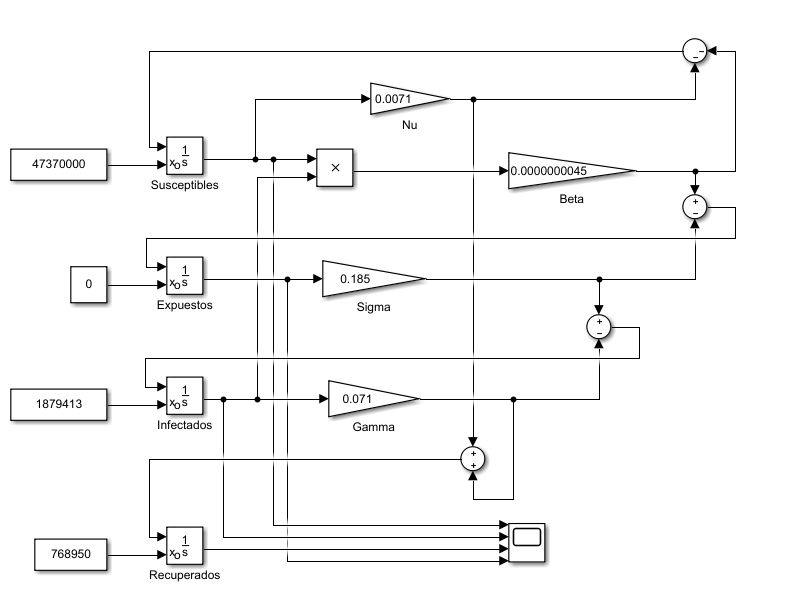
\includegraphics[width=0.7\textwidth]{img/modelo_SEIRV.png}
        \caption{Diagrama de bloques en Simulink para el modelo SEIRV}
        \label{fig: diagrama de bloques en Simulink para el modelo SEIRV}
        \vspace{0.5cm} % Ajusta el espacio vertical entre la imagen y el texto
\end{figure}


\section{Diseño arquitectónico}
El sistema desarrollado consta de tres componentes principales:

\begin{itemize}
    \item \textbf{Modelos en Simulink:} cada modelo epidemiológico se implementa mediante diagramas de bloques que representan las ecuaciones diferenciales del sistema. Esto permite simular la dinámica de la epidemia de manera visual e intuitiva.

    \item \textbf{Scripts en MATLAB:} se utiliza para la implementación del controlador PID en el modelo SIR, actuando sobre la tasa de transmisión para mitigar la propagación.

    \item \textbf{Interfaz gráfica en App Designer:} diseñada para permitir al usuario modificar parámetros epidemiológicos y del controlador, ejecutar simulaciones y visualizar resultados de forma interactiva mediante gráficas dinámicas.
\end{itemize}


No se han desarrollado diagramas de clases ni de despliegue, dado que el proyecto no utiliza programación orientada a objetos ni arquitectura distribuida. La estructura es modular, basada en scripts, modelos de Simulink y la aplicación gráfica integrada.

